% Created 2025-01-09 Thu 22:53
% Intended LaTeX compiler: pdflatex
\documentclass[11pt]{article}
\usepackage[utf8]{inputenc}
\usepackage[T1]{fontenc}
\usepackage{graphicx}
\usepackage{longtable}
\usepackage{wrapfig}
\usepackage{rotating}
\usepackage[normalem]{ulem}
\usepackage{amsmath}
\usepackage{amssymb}
\usepackage{capt-of}
\usepackage{hyperref}
\author{Akilan}
\date{\today}
\title{}
\hypersetup{
 pdfauthor={Akilan},
 pdftitle={},
 pdfkeywords={},
 pdfsubject={},
 pdfcreator={Emacs 29.1 (Org mode 9.6.6)}, 
 pdflang={English}}
\begin{document}

\tableofcontents

\section{Evaluation}
\label{sec:org02aba25}

We conducted tests of the FAT Pointer-based range addresses against Jemalloc, 
the default memory allocator for CHERIBSD(, ), to assess the performance improvements 
enabled by a CHERI-based huge page-aware allocator. Specifically, we evaluated 
the reduction in TLB misses and its impact on overall 
performance metrics, such as wall clock runtime.

To comprehensively analyze the proposed allocator, we categorized benchmarks into 
two classes which are micro and macro benchmarks. Micro benchmarks comprise smaller 
C programs designed to target specific allocator patterns, enabling us to evaluate 
detailed aspects of the allocator's behavior. Macro benchmarks, on the other hand, 
encompass larger, real-world C programs, allowing us to assess the allocator's 
performance in more practical, real-world scenarios.

The experiment setup details the software stack used for evaluation. It includes 
the specific configurations, compiler options, and system environment tailored 
to benchmark the proposed allocator. This ensures consistency and repeatability 
in our results, providing a solid foundation for meaningful comparisons.

We further elaborated on the two classes of benchmarks executed. Micro benchmarks 
focused on particular allocation and deallocation patterns, such as sequential and 
random memory accesses, to stress-test the allocator under controlled conditions. 
Macro benchmarks involved real-world applications, offering insights into how 
the allocator performs with complex memory allocation demands, large datasets, 
and varying execution contexts.

The results section presents the outcomes of our benchmarks, highlighting key metrics 
such as TLB miss rates, memory usage, and runtime performance. We observed that the 
proposed allocator demonstrated significant improvements in reducing TLB misses, 
leading to noticeable enhancements in runtime efficiency for both micro and macro 
benchmarks. The behavior of specific allocation patterns and their impact on memory 
performance is detailed, providing a nuanced understanding of the allocator's effectiveness.

Based on the evaluated results, the usability of the proposed allocator shows promise 
for applications requiring optimized memory management and reduced overhead from TLB misses.
However, limitations were also identified, such as scenarios where the allocator's performance 
gains were marginal or where it introduced additional complexity in memory management. These 
limitations provide a roadmap for future optimizations and refinements of the allocator design.

\subsection{Expirement setup}
\label{sec:org9bf5b27}

The CHERI Morello board was used to evaluate the proposed memory allocator. 
Morello implements the ARM A76 with enhanced server-class memory, featuring a 
quad-core ARM CPU with capability extensions. The L1 and L2 caches were modified 
to proliferate the capability bit, ensuring compatibility with CHERI's capability-based 
memory model. When compiling the C programs for benchmarking, the Benchmark ABI was 
used as recommended by the CHERI community. This compilation mode was enabled using 
the Clang compiler.

The Benchmark ABI was specifically designed because the Morello branch predictor 
was not expanded to predict bounds. Consequently, a capability-based jump introduces 
stalls in later PCC-dependent instructions until bounds are established. This issue 
is particularly significant during dynamically linked calls and returns between 
libraries, where bounds are changed to cover the called or returned-to library. 
Such stalls can negatively affect performance, making the Benchmark ABI an essential 
consideration for this evaluation.

Each C program was executed using two different memory allocators. The first was 
the modified C allocator, imported as a header file. This approach was necessary 
because the Benchmark ABI shared object file exhibited unexpected behavior, 
failing to overwrite the C program at runtime with the intended malloc functions. 
The second allocator was the standard OS memory allocator, which, in the case of
CHERIBSD, is Jemalloc.

Performance measurements were carried out using ARM performance counters to 
ensure accurate evaluation. These counters provided detailed metrics, allowing 
us to compare the performance of the two allocators and assess the impact of 
the proposed changes.

\subsubsection{Performance counters used}
\label{sec:org294979c}

\begin{center}
\begin{tabular}{|l|l|}
\hline
Performance counter & Description \\
\hline
Wall clock & The actual time taken from the start of a \\
 & computer program to the end. \\
 & \\
(p/l1d\_tlb\_rd) L1 data TLB reads & Level 1 data TLB access, read \\
 & \\
(p/l2d\_tlb\_rd) L2 data TLB reads & Level 2 data TLB access, read \\
 & \\
(p/l1d\_tlb\_refill) L1 data TLB refills & Level 1 data TLB refill. \\
 & The Level 1 data TLB refill \\
 & counter tracks each access to \\
 & the L1D\_TLB that results \\
 & in a refill of the Level 1 data \\
 & or unified TLB. This includes any \\
 & access that requires a memory lookup \\
 & due to a translation table walk \\
 & or accessing another level of TLB cache. \\
 & \\
(p/cpu\_cycles) CPU cycles & The CPU CYCLES counter increases with \\
 & every clock cycle. However, it can be \\
 & affected by changes in clock frequency, \\
 & such as when WFI (Wait for Interrupt) \\
 & or WFE (Wait for Event) \\
 & instructions pause the clock. \\
 & \\
(p/dtlb\_walk) Data TLB walks & Data TLB access with at least \\
 & one translation table walk. \\
 & \\
(p/ll\_cache\_miss\_rd) Last level cache miss reads & Last level cache miss, read \\
 & (This refers to every miss in the \\
 & Last level cache that occurs \\
 & during a memory read operation.) \\
\hline
\end{tabular}
\end{center}

\subsubsection{Benchmarks}
\label{sec:orgddacffd}
The benchmarks are classified into 2 classes:

\begin{enumerate}
\item Micro benchmark
\label{sec:orgb329a4e}
\begin{itemize}
\item GLIBC: The Glibc benchmark evaluates the performance of
malloc and free functions in single-threaded, multi-threaded,
and emulated multi-threading scenarios using various block sizes and
allocation patterns. It simulates real-world memory usage by partially
deallocating blocks in FIFO order and fully deallocating them in LIFO order.
Results are gathered across configurations to analyze performance variations.
\item MemAccess: This benchmark by Alex Bordei evaluates the performance impact of
memory access patterns by constructing and traversing a doubly
linked list with varying working set sizes. It supports sequential or
randomized structures, optional node operations, and multithreaded
traversal using pthreads. The program dynamically allocates memory and systematically
doubles the working set size to analyze memory hierarchy behavior.
\end{itemize}

\item Macro runs
\label{sec:orga786fd0}
\begin{itemize}
\item Kmeans: Kmeans implements a parallelized K-means clustering algorithm that
assigns data points to clusters based on proximity to centroids,
iteratively updating them until convergence. The computation is
distributed across threads using the pthread library, dynamically
assigning tasks to optimize performance. Parameters like data size
and clusters are configurable, and the program ensures efficient
memory management and synchronization.
\item Richards: Richards is a task scheduling benchmark that simulates a
multitasking environment with tasks of varying types and priorities,
communicating through queued packets. The schedule function manages
task execution based on state and priority, tracking processed packets
and held tasks for performance evaluation. Configurable iterations and
timing help measure system performance and ensure correctness.
\end{itemize}
\end{enumerate}

\subsection{Results}
\label{sec:org4bdc0d9}
\begin{center}
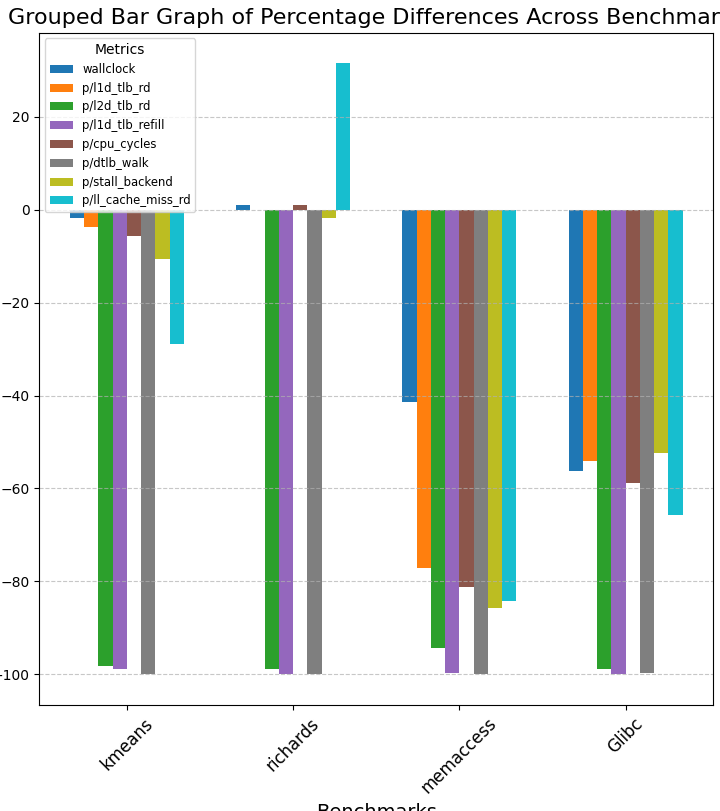
\includegraphics[width=.9\linewidth]{./diagrams/allbenchmarks.png}
\end{center}

\begin{center}
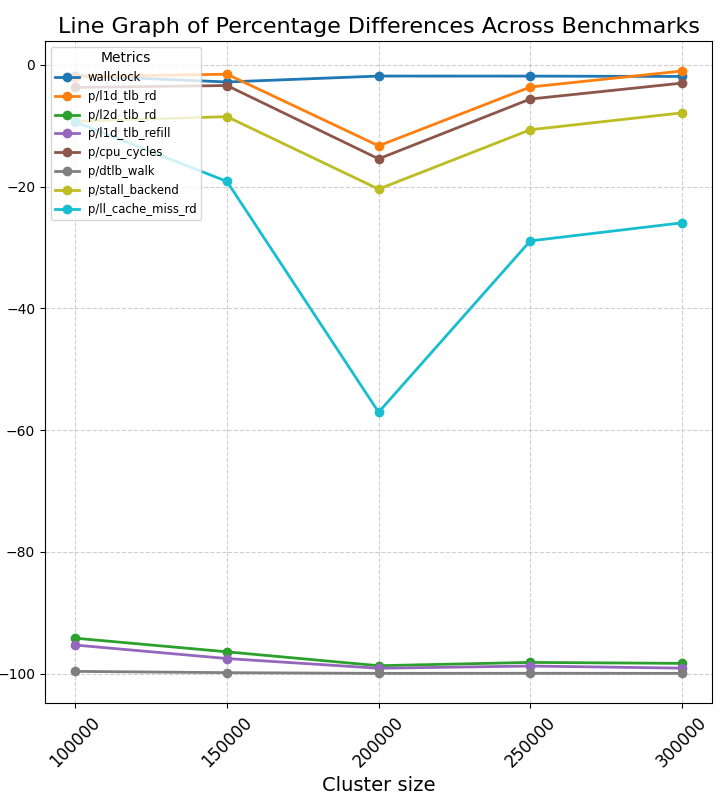
\includegraphics[width=.9\linewidth]{./diagrams/kmeans.png}
\end{center}

\begin{center}
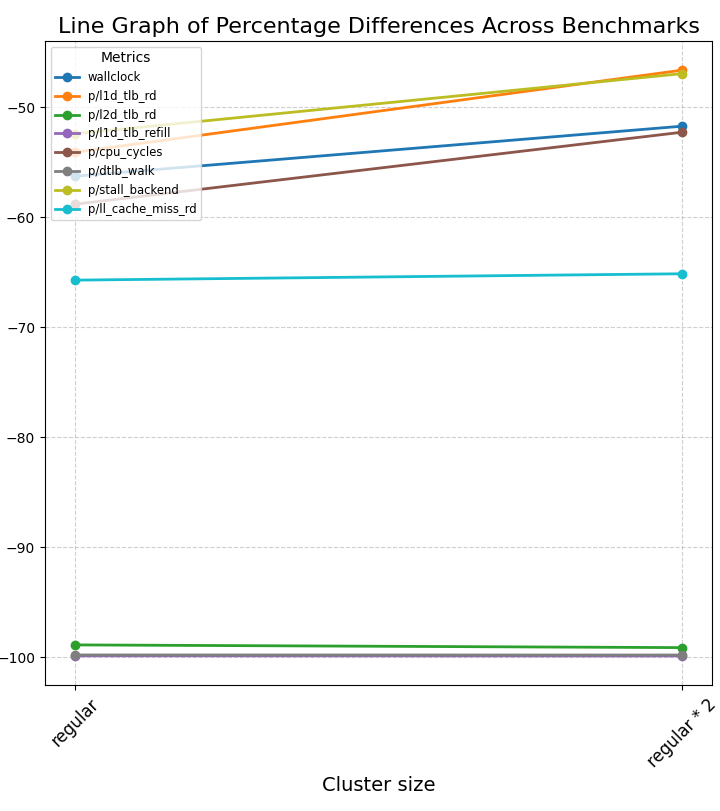
\includegraphics[width=.9\linewidth]{./diagrams/glibc.png}
\end{center}

\subsection{Usability}
\label{sec:org3b91bbd}
\end{document}